%!TEX TS-program = XeLaTeX
\documentclass[12pt]{article}
\usepackage[top=1in, bottom=1in, left=1in, right=1in]{geometry}

%%%
%% Needed for fonts in xelatex to work
%%%
% NOTE: I actually use XeLaTeX, which allows me to get the fonts
% exactly the way that I want them. For proposals, this means
% I can use Times New Roman instead of the default Computer
% Modern. I actually like Computer Modern, but since Arial
% is what the solicitation suggests there's no point in throwing off a reviewer
% with an unexpected font, particularly one with such a
% polarizing reaction in readers. Never upset the reviewrers, I
% always say.
%
% What's the point of this bit of rambling? If you do not want to use
% XeLaTeX and would rather stick to good old LaTeX, then you
% need to comment out the next few lines of font packages and
% font commands.
%
% If you want to use XeLaTeX but want different fonts, then you
% just need to change the name in the argument for \setmainfont.
% Make sure that the font you use is loaded on
% your machine and your TeX distribution knows how to find it.
% See Google if you need to learn more about this.
%
\usepackage{fontspec}
\setmainfont{Arial}

%%%
%% Packages that I use on a regular basis.
%%%
% Of course, you are likely to need some math typesetting so these
% three packages have you covered.
\usepackage{amssymb}
\usepackage{amsmath}
\usepackage{latexsym}
% I use color, graphicx, and epstopdf to read in PDFs for my figures.
\usepackage{color}
\usepackage{graphicx}
% \usepackage{epstopdf}
% I don't remember why threeparttable and setspace is here. Inertia.
\usepackage{threeparttable}
\usepackage{setspace}
%\doublespacing
%%%
%% Some packages to handle the figures and captions
%%%
\usepackage[labelfont=bf]{caption}
\usepackage{subcaption}
\usepackage{wrapfig}

%%%
%% Packages and settings for my bibliography.
%%%
% apa_with_doi is a style I created to keep DOI in the bibliography
% but strip out URLs. There are a lot of other styles you can
% find for natbib. Again, Google is your friend.
% Author name and year references, i.e., Author (year):
%\usepackage{natbib}
%\bibliographystyle{apa_with_doi}
% Numbered references:
\usepackage[numbers,super]{natbib}
\bibliographystyle{unsrtnat}


%%%
%% Packages and commands to build my table of contents (TOC).
%%%
%% The trick was getting the References included properly.
%% Also, some of my table of contents entry have no page number
%% because those pages are generated separately by my institute.
%% Nothing to be done about that. You may or may not have the
%% same problem, so you may or may not have to tweak this.
\usepackage[nottoc,numbib]{tocbibind}
\renewcommand{\tocbibname}{References\setcounter{page}{1}}
\usepackage{tocloft}
\renewcommand{\cftsecleader}{\cftdotfill{\cftdotsep}}

%%%
%% These commands get the spacing around the title and section titles right.
%%%
% I tightened up the spacing. The LaTeX default is just too roomy.
% This spacing is still clean and legible, just not so free with the
% whitespace between sections.
%
% First the title.
\usepackage{titling}
\setlength{\droptitle}{-50pt}
\pretitle{\begin{center}\Large\bfseries\vspace{0ex}}%
\posttitle{\end{center}\Large\vspace{-2ex}}%
\preauthor{\begin{center}\large}%
\postauthor{\end{center}\large\vspace{-3ex}}%
\predate{\begin{center}\large}%q
\postdate{\end{center}\large\vspace{-6ex}}%
% Now the section headings.
\usepackage[noindentafter]{titlesec}
\titleformat{\section}{\large\bfseries}{\thesection}{1em}{}
\titlespacing{\section}{0pt}{18pt plus 2pt minus 2pt}{4pt plus 2pt minus 2pt}[0pt]
\titlespacing{\subsection}{0pt}{16pt plus 2pt minus 2pt}{4pt plus 2pt minus 2pt}[0pt]
\titlespacing{\subsubsection}{0pt}{14pt plus 2pt minus 2pt}{4pt plus 2pt minus 2pt}[0pt]

%%%
%% These commands get the lists to work the way that I want them to.
%%%
% i.e. I want less space wrapping around the list.
\usepackage{enumitem}
\setlist{nolistsep}
\setlist[2]{noitemsep}
\setlist[1]{noitemsep}

%%%
%% Commands for making the tables.
%%%
\usepackage{booktabs}
\usepackage{multirow, hhline}
\usepackage{array}
\usepackage[table]{xcolor}% http://ctan.org/pkg/xcolor

%%%
%%% Package to create Gantt schedules
%%%
\usepackage{pgfgantt}


%%%
%%% Formatting urls
%%%
\usepackage{url}
\urlstyle{rm}

%% The lineno packages adds line numbers. Start line numbering with
%% \begin{linenumbers}, end it with \end{linenumbers}. Or switch it on
%% for the whole article with \linenumbers after \end{frontmatter}.
\usepackage{lineno}

%% In order to have a caption to the side of a figure or table, use the
%% 'sidecap' package.
\usepackage[rightcaption]{sidecap}
\sidecaptionvpos{figure}{t}

\usepackage{wrapfig}


%% For more control of the enumeration environment (lists with numbers)
%% use the enumitem package.
%\usepackage{enumitem}

%% Also, to reset the numbering of enumerate, use the following:
%\setenumerate[0]{label=\alph*.}

% To deal with figures all alone on a page.
\renewcommand{\floatpagefraction}{.8}%

% To use symbols for the footnotes:
\renewcommand{\thefootnote}{\fnsymbol{footnote}}

% set up the page numbers as 1-N, 2-N, ...
\numberwithin{page}{section}
\renewcommand{\thepage}{\thesection-\arabic{page}}

% https://tex.stackexchange.com/questions/210871/latex-page-numbering-by-section
%this does not seem to work, just hard code it :(
% not sure if there is something else in this template that is breaking it
% or things have changed in the last 6 years?
%\usepackage{etoolbox}
%\makeatletter
%% Make sure that page starts from 1 with every \section
%\patchcmd{\@sect}% <cmd>
%  {\protected@edef}% <search>
%  {\def\arg{#1}\def\arg@{section}%
%   \ifx\arg\arg@\stepcounter{page}\fi%
%   \protected@edef}% <replace>
%  {}{}% <success><failure>
%\makeatother
\makeatletter
\renewcommand{\paragraph}{%
  \@startsection{paragraph}{4}%
  {\z@}{1.25ex \@plus 0ex \@minus .2ex}{-.5em}%
  {\normalfont\normalsize\itshape\bfseries}%
}
\makeatother
%% Finally, we get to the document.
\begin{document}
\title{Revamping Matplotlib for Modern Data Structures}
\author{Thomas A.\ Caswell}
\date{}
\maketitle

% First, let's get that TOC in there. NASA likes it.
\setcounter{tocdepth}{2}
\tableofcontents
\thispagestyle{empty}
% Let's leave this TOC alone on this page and start a new one for
% proposal body.
\newpage

\section{Scientific/Technical/Management (S/T/M)}
% Let's reset the page counter.
\setcounter{page}{1}
% the subsection are a combination of the lines labeled "Content" in
% Table 1 (on ROSES-20 SoS-51) and the text in E.7.3 (on E.7-2 -
% E.7-3) describing what needs to be in the proposal.

% not sure that this order is right, but I think we need to hit all of
% these points.  Maybe want to rename the section headings or merge
% some of them?
\subsection{Matplotlib's role in scientific computing}

Matplotlib~\cite{Hunter:2007} is a comprehensive Python library for
creating static, animated, and interactive visualizations.  It
provides the visualization for projects across all SMD divisions,
including flagship missions like the Hubble Space Telescope (HST) and
the James Webb Space Telescope~\cite{jwst_pipeline} (JWST), and
instruments like the Curiosity Rover
Mastcam~\cite{https://doi.org/10.1002/2016EA000219}.

Matplotlib is part of the Scientific Python Ecosystem (SPE), a loosely
defined community of projects and programmers with the common goal of
advancing science through the use of the Python programming language.
This development is largely volunteer work or work that is sponsored
implicitly by specific science projects.  SPE, shown with a rough
schematic in Figure \ref{fig:ecosystem}, has a core of general purpose
domain-agnostic tools, like NumPy~\cite{Harris2020} and
SciPy~\cite{Virtanen2020}. Matplotlib is in the next ring of
specialized, but still domain agnostic tools, and is the most
prevalent data visualization library for the SPE.  The outer rings are
increasingly domain-specific tools, like
AstroPy~\cite{astropy:2013,
  astropy:2018} for astrophysics,
SunPy~\cite{sunpy_community2020}  for heliophysics, and
MetPy~\cite{metpy} and cartopy~\cite{Cartopy} for earth sciences; all of these use
Matplotlib for specialized plotting.  This layered approach gives
scientists and engineers convenient and powerful high-level tools
while enabling direct access to the underlying libraries when needed.


\begin{wrapfigure}{r}{0.5\textwidth}
  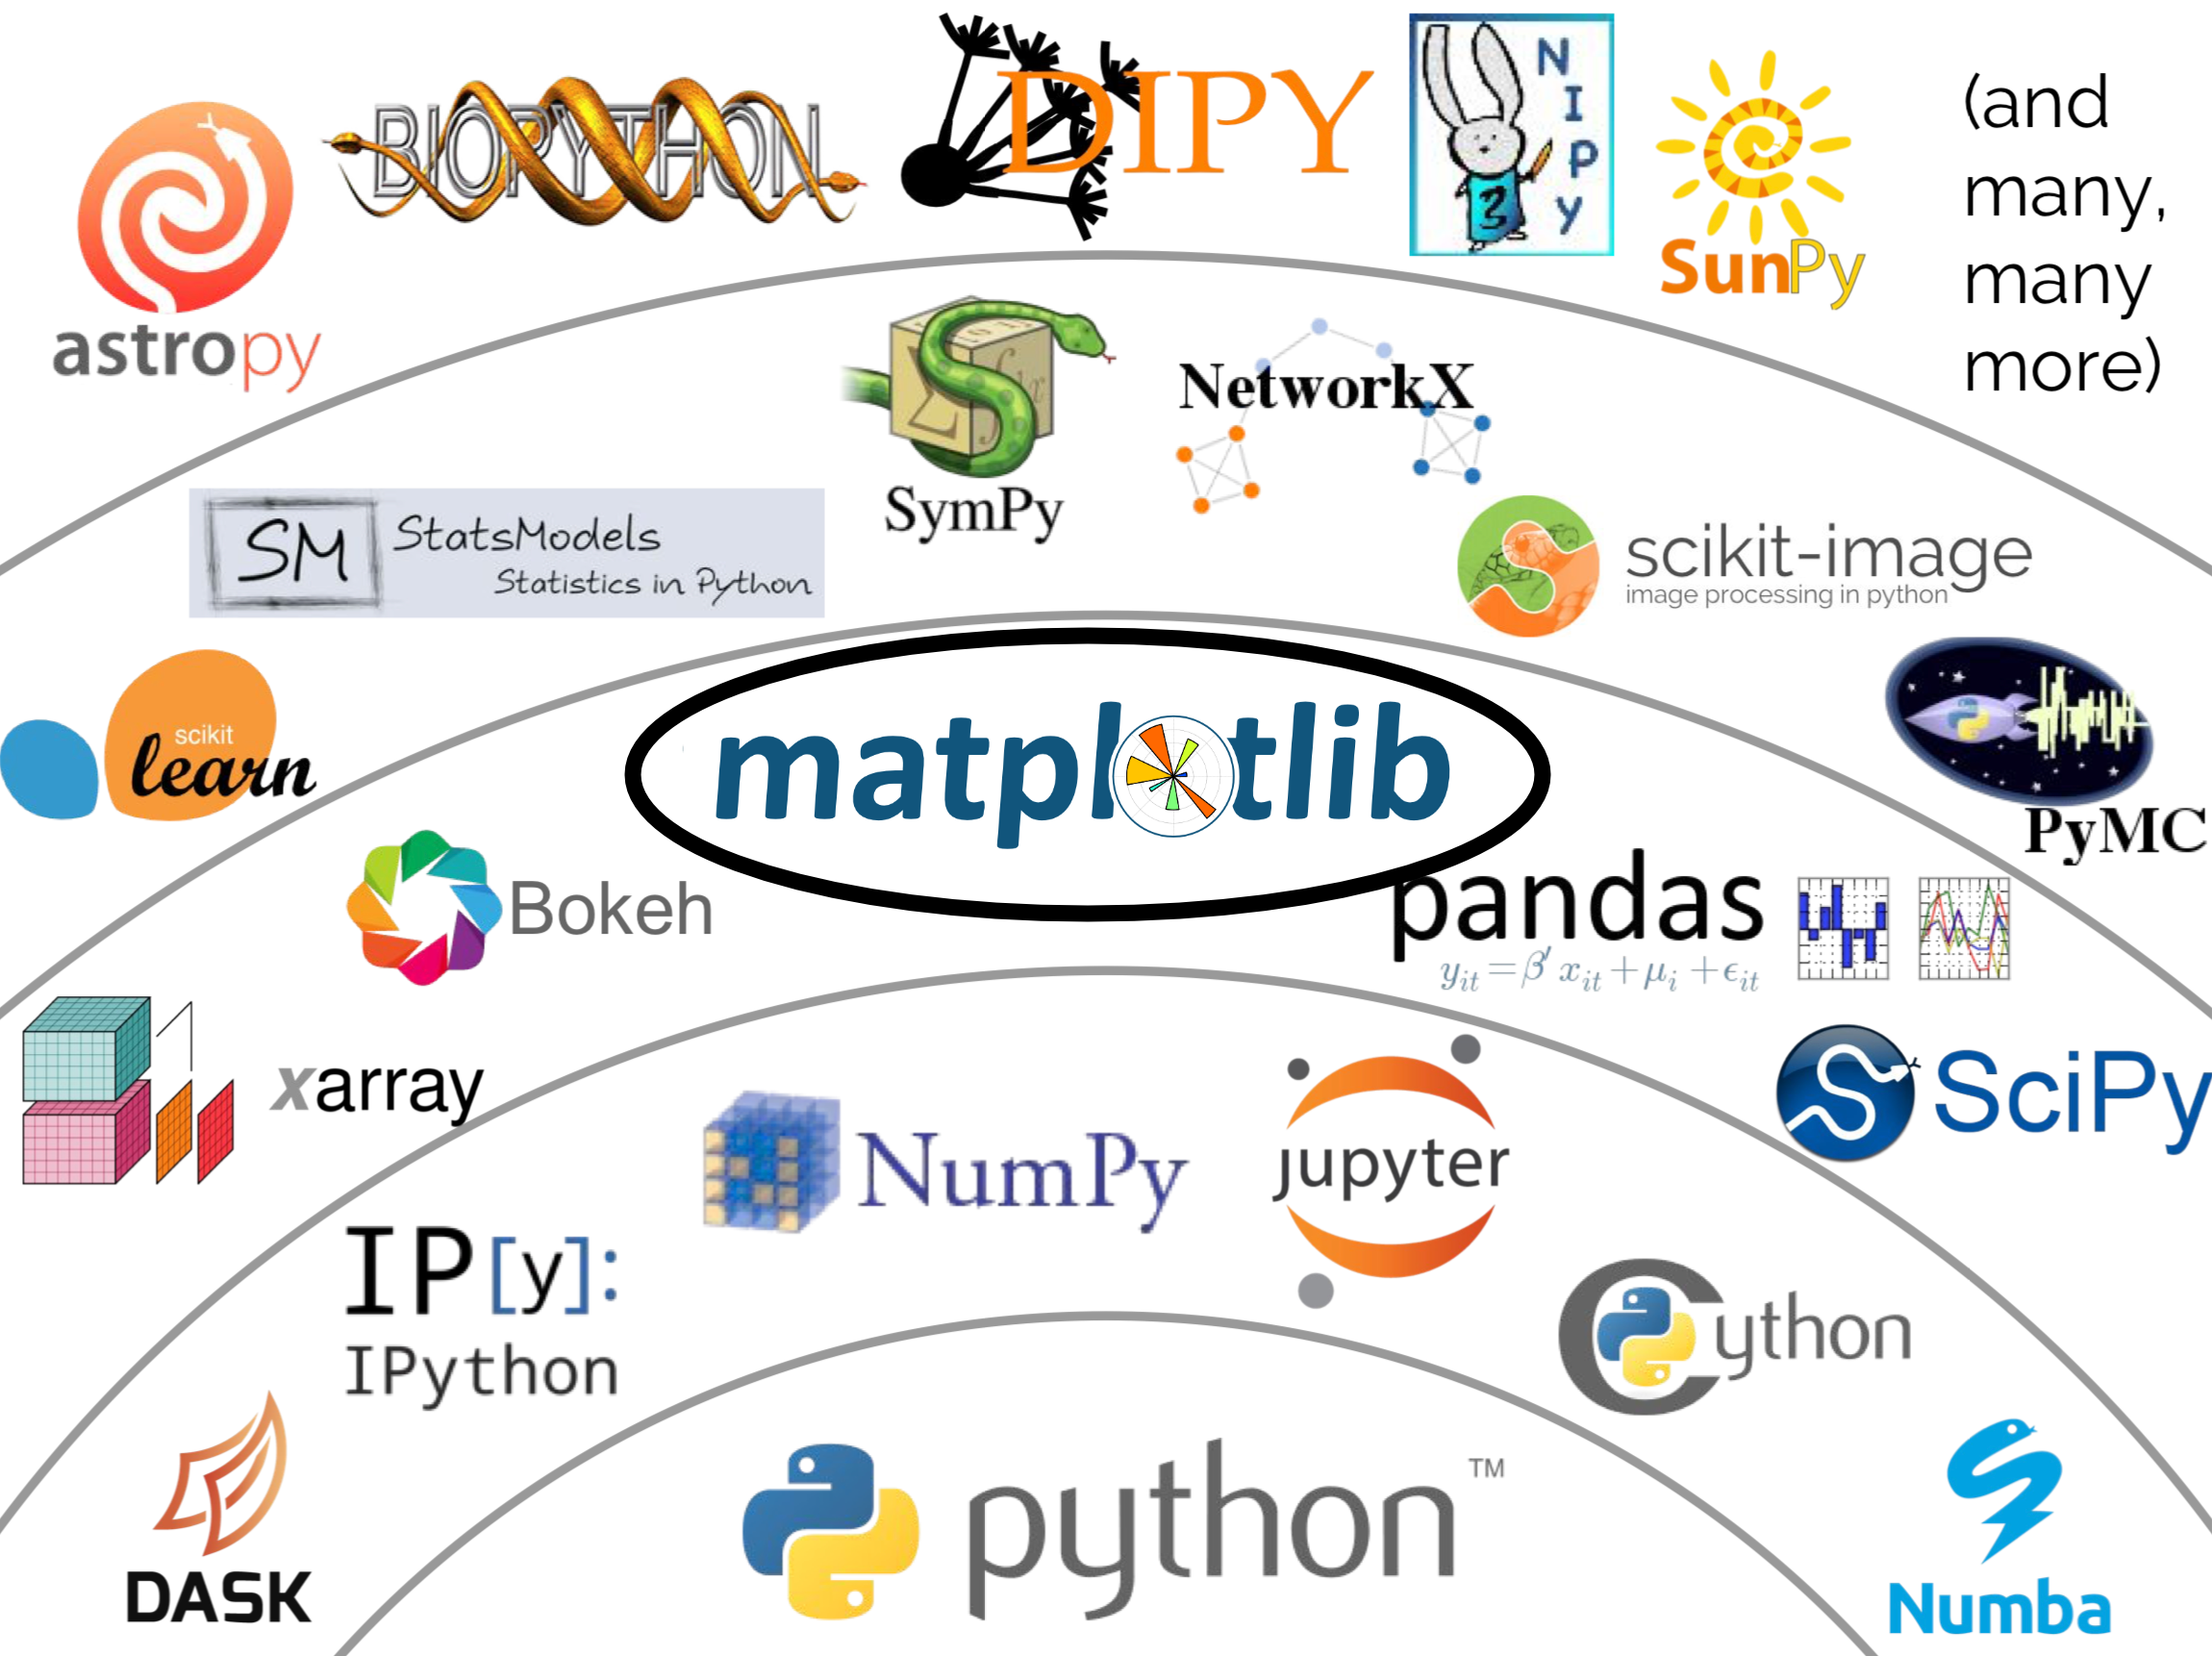
\includegraphics[width=0.45\textwidth]{scipy-ecosystem}
  \caption{\small A schematic of the Scientific Python ecosytem.  At the
    core we have the Python language itself with concentric rings of
    domain agnostic to domain specific libraries.  Both AstroPy (top
    left) and SunPy (top right), used in the astrophysics and
    heliophysics divisions respectively, rely on Matplotlib (center, circled)
    Credit: Jake van der Plas, ``The Unexpected Effectiveness of Python
    in Science'', PyCon 2017}
  \label{fig:ecosystem}
\end{wrapfigure}


Soon after its start by John D. Hunter in 2002, Matplotlib began growing as an
open source plotting
library with a BSD-compatible license. The
first commits in the Matplotlib history date to early 2003.  Over the
last 17 years Matplotlib has been actively developed and maintained by
a vibrant, primarily volunteer, community.  Matplotlib has over 1,250
individual contributors to the code base, with many more individuals
having contributed in ways not easily tracked, such as answering user
questions on the mailing list and reporting issues.

Matplotlib has a high-level API for quick plotting, such as in
exploratory data analysis, plus a low-level API that gives full control for
fine-tuned publication-quality plots, for animations, for writing both
GUI-independent and GUI-specific tools for interactive data plotting, and
for output to a variety of vector and raster
formats including \texttt{svg}, \texttt{eps},
\texttt{pdf}, and \texttt{png}.

Matplotlib's generality and flexibility make it readily extendable to
many data visualization domains.  A rich ecosystem of downstream packages use
Matplotlib as their base, providing domain-specific streamlining of
Matplotlib's API: including
yt~\cite{2011ApJS..192....9T}, AstroPy~\cite{astropy:2013,
  astropy:2018}, ArviZ~\cite{arviz_2019},
seaborn~\cite{waskom2020seaborn}, xarray~\cite{hoyer2017xarray},
cartopy~\cite{Cartopy}, corner.py~\cite{corner} and
mpl-scatter-density~\cite{mpl-scatter-density}.

Matplotlib is ubiquitous in scientific computing.  Conservative
estimates based on downloads and on usage of the documentation website
indicate that Matplotlib has over a million users.  We expect that a
large fraction of NASA SMD-sponsored projects rely on this shared
infrastructure to some degree, but this is hard to quantify.
It is not usual to cite tool chains in scientific literature, so
citation counts are likely to vastly under-represent the scientific
use of Matplotlib.  For example, a canonical reference for
Matplotlib~\cite{Hunter:2007} has over 12,750 citations overall and
over 4,500 citations in ADS~\cite{ads_mpl},
while a common reference of NumPy~\cite{walt2011numpy} has over 6,800
citations. These counts illustrate the problem in measuring usage via
citations: Matplotlib depends on NumPy, yet Matplotlib has almost
twice as many citations.

\subsection{Objectives}

% - need to re-engineer Matplotlib's data model
% - have on-going work to do design and prototypes
% - need significant SEW effort to implement across whole library
% - one nice thing is units, focus on documenting / planning / testing
% - another nice thing is resampling and out-of-core data access
% - we have to do this while keeping the patient writing papers


Matplotlib is a primarily community-driven project, but we have grown
to the point where we need supported developers with the time to
organize, plan, and make decisions.  Supported developers will allow
us to take on more complex projects than can be implemented by part-time
volunteer effort alone, while executing critical day-to-day
maintenance tasks required to keep the project healthy.
\textbf{We propose to split the effort on this grant equally between
  the two primary activities: overhauling our internal data representation, and library
  maintenance}.


\subsubsection{Refactor the Internal Data Model}
\label{sec:ridm}

Matplotlib is based on visualizing data stored in Numpy arrays,
which is a simple yet flexible data model that has been the
underpinning of data visualization for the last few decades.  However,
new data types are being developed and standardized to carry
structure and metadata along with the numerical values of the data.
Physical units are a key example of such metadata
that a plotting package should handle gracefully.  Modern data
structures can also describe massive data sets and allow performing
operations without loading the whole data set into memory
(i.e. dask, xarray); Matplotlib should leverage these packages
to work efficiently with Big Data.

Eliding many of the implementation details, Matplotlib can be thought
of as having three primary layers~\cite{AOSA_mpl}: the user-facing plotting
methods; the \texttt{Artist} layer; and the backends.  The core of the
architecture is the set of \texttt{Artist}s which can be understood as
objects that describe something for a backend to render to the output device.
Each individual
\texttt{Artist} is responsible for holding the user data and style
information for part of the final visualization, but the exact data
held varies among \texttt{Artist} classes.  For example,
\texttt{matplotlib.text.Text} is responsible for drawing text and
holds, among other things, the location of the text, the font family
and size, the color, and the actual string.  Internally Matplotlib
represents a \texttt{Figure} as a tree of \texttt{Artist}s.  The
plotting methods in Matplotlib create these objects and add them to
the tree.  To render the final output Matplotlib walks the
\texttt{Artist} tree depth-first and each each \texttt{Artist} is
responsible for rendering itself via the backend.  Thus, by changing
the backend we can change the output format from raster to vector
without making any changes to the \texttt{Artist} tree.


Currently, each plotting method and \texttt{Artist} independently
handles sanitizing and storing data.  Hence, each \texttt{Artist}
subclass holds its data in a different way and some common
functionality, such as handling data with attached units (e.g.,
degrees Celsius, dates), is repeated throughout the code base.  This
leads to inconsistencies across the library and makes it difficult for
users to write code that updates interactive explorations or
animations.  Another consequence of the data storage is that
Matplotlib also cannot exploit ``Structured data''--combining multiple
pieces of (possibly heterogeneous) data with labels and metadata into
single data structure; instead, users must extract data elements and
reassemble them as arguments to Matplotlib plotting functions.

We have on-going theoretical and design work\footnote{Supported by the
Chan Zuckerberg Initiative, see current support.} to re-architect
Matplotlib to better separate the data representation from the rest of
the library.  We are developing a consistent data access API such that
each \texttt{Artist} will have a single \texttt{DataSource} object
responsible for providing access to all of the data that the
\texttt{Artist} needs.  This design will allow us to overcome many of
the issues with the current design, opening the door to
new functionality.  The current work is expected to produce design
documents and a proof-of-principal implementation by the end of 2021.
Based on this preliminary work \textbf{we propose refactoring all of
  Matplotlib to use the new data model}.  The proposed design is
consistent with the rest of the architecture; just as the
\texttt{Artist}s are currently agnostic to the backend used, the
\texttt{Artist}s will be agnostic to the internals of its \texttt{DataSource}.

An immediate motivation for this refactor is to improve
Matplotlib's handling of data with physical units attached.  Units are
fundamental to science and engineering, but most numerical
software is unit-naive.  It is the user's responsibility to
convert data to consistent units prior to any
computation.  Failing to do so leads to the most insidious of bugs:
everything ``works'' but silently gives incorrect results!  There are
several libraries which provide unit-aware data structures in Python
that can be used with Matplotlib for unit-aware plotting.
\textbf{This capability is currently used to support spaceflight
  operations by Monte, JPL's mission design and navigation software
  system}; NASA supported its initial development in Matplotlib.



% to what extent mpl currently supports units

The current support for physical units in Matplotib is based on
inspecting the incoming data type.  When the the data structure supplied by
the user includes units, Matplotlib looks for a registered converter and sets
default axis labels, limits, and functions for locating and formatting
the ticks.  Internally, Matplotlib uses the unit machinery to handle
datetime and string-categorical types. Third-party libraries are
able to register their own converters.  With this machinery users can
control the units in which the data is plotted, which may differ from
the units in which it was supplied.  Axis limits may be specified
in physical
units.

% what is wrong
There are several problems with the current unit support in
Matplotlib.  It is under-documented, making it hard for users to
understand and use, and hard for developers to extend.  Test
coverage is incomplete, and inconsistencies have accumulated in the
code base.  These range from subtle inconsistencies between plotting
methods to data with units simply not working with some methods.
\textbf{To address this we propose to use unit-handling as a
  motivating feature while doing the \texttt{DataSource} refactoring}.
Unit logic will be consolidated in the \texttt{DataSource}.
% By implementing all of the unit logic in the \texttt{DataSource} we
% will be able to share the code across all \texttt{Artist}s and unify
% how we treat units across the library.
%% The original sentence was confusing to me, and, I think, unnecessary.

There is a broad recognition across the SPE of the importance of
supporting physical units as an intrinsic component of computation.
There is on-going work in NumPy (NEP40-43), pandas, and xarray to add
support for physical units to their foundational data structures.  The
proposed work will ensure that Matplotlib can take advantage
of such efforts, for seamless handling of data with units from computation
to visualization.

In addition to fixing problems with the current
support of physical units, this refactoring will lay the ground work for
\begin{itemize}[noitemsep]
  \item smart down-sampling of plotted data based on view limits,
  \item native consumption of structured data,
  \item seamless updating of the underlying data, either interactively
    or via streams,
  \item and use of alternative data sources such as out-of-core data
    structures, database queries or analytic functions.
\end{itemize}

\subsubsection{General maintenance}

While rewiring Matplotlib's data model,
we need to sustain Matplotlib as a vibrant project and
continue to support the hundred of thousands of users and hundreds of
downstream packages.  To maintain Matplotlib's health we must:
\begin{itemize}[noitemsep]
\item fix critical bugs and regressions promptly as they are reported;
\item make improvements while maintaining backward compatibility and
  documenting changes;
\item categorize Issues and PRs in terms of topic, difficulty, and
  urgency;
\item entrain new contributors to sustain and diversify the community
  developer team;
\item maintain the continuous-integration infrastructure;
\item manage the release process;
\item and manage community discussions about proposed enhancements, features,
  and API changes.
\end{itemize}
These are tasks that are never ``done''; users find new ways to use
the library, they expose previously un-detected bugs, they request or propose new
features, and the world continues to changes around us.   \textbf{Dedicated
full-time developers help ensure that things happen in a consistent and timely
manner, and provide the crucial roadmaps that will steer the future of the library}.


%plot?

Historically, pull requests (PRs) and issues have been submitted
faster than they can be reviewed; Matplotlib has accumulated about 300
open PRs and 1300 open issues due to this imbalance. There are
critical bug reports and insightful feature requests among the issue
backlog, while among the PR backlog there are useful contributions or
bug fixes that would improve the libraries for direct users and
downstream packages.  The large backlog is discouraging for new and
occasional contributors and distracting for core developers.

In 2020, with a grant from CZI supporting a Research Software Engineer
(RSE) working on Matplotlib for 10 month, we resolved 2,056 PRs and
999 issues.  However, even at this rate we only reduced the PR backlog
by 70 open PRs and held the issue backlog even.  As part of reducing
the backlog, we were able to fix several long-standing bugs.  We have
demonstrated that supporting maintenance work has a positive effect on
the health of the project and \textbf{the additional resources
  requested here will further reduce, but not eliminate, the
  maintenance backlog}.



\subsection{Impact and Relevance to Science Mission Directorate}

As mentioned above, it is hard to estimate the prevalence of open
source software due to it being freely distributed and not
systematically cited.  Matplotlib is in the top 100 most-downloaded
packages from PyPI~\cite{pypi_stats} and is packaged by every major
Linux and scientific Python distribution.  Another metric to measure
impact is static analysis of publicly available code.  According to
github over 299k repositories and over 12k packages hosted on GitHub
depend on Matplotlib~\cite{gh_deps:2021}. A recent study of the
almost 10M Jupyter notebooks on github found that over 3M of them have
a direct Matplotlib import~\cite{datalore:2020}.

These measures show broad impact but cover many uses outside of the
SMD community.  If we restrict the static analysis to
\url{https://github.com/nasa}, NASA's official organization on GitHub,
we see that 53 of the 330 hosted repositories make reference to
Matplotlib.  Soliciting on social media for examples of Matplotlib in SMD research
yielded a (non-exhaustive) list including:
\begin{itemize}[noitemsep]
\item
  to study
  thunderstorms~\cite{https://doi.org/10.1002/2016JD025299,https://doi.org/10.1029/2019JD030874},
  seasonal ocean winds~\cite{https://doi.org/10.1002/2017JD027516} and
  tropical storms~\cite{Lang_2020};
\item in the first science paper from the Parker Solar
  probe~\cite{Bale2019};
\item in the Martian science program in both
  orbiter~\cite{https://doi.org/10.1029/2019JE006188} and
  rover~\cite{https://doi.org/10.1002/2016EA000219} contexts;
\item as part of ground operations from the Mars Phoenix Lander;
\item with data from Kepler and K2 missions to study Trojan
  asteroids~\cite{Nixon_2019} and
  Titan~\cite{Ryan_2017,2019PASP..131h4505P};
\item on the New Horizons Kuiper belt extended
  mission~\cite{Porter_2018};
\item for visualization of scheduling, safety and constraint checks,
  and telemetry by the Swift science operations
  team~\cite{swift_ops,2020ApJ...900...35T};
\item as part of the HST and JWST~\cite{jwst_pipeline} data processing
  pipelines;
\item in Monte, JPL's mission design
  and navigation software system to support spaceflight operations;
\item in fundamental research on graphene~\cite{PhysRevLett.120.236802};
\item and for work on nuclear powered rockets~\cite{leu_cerment}.
\end{itemize}
This list shows the breadth Matplotlib usage across the SMD
divisions.  \textbf{Small investments in Matplotlib will have returns across
the entire SMD portfolio}.

Maintaining Matplotlib's health and engineering for its future will
have wide-ranging impacts for the scientific community, and for NASA in
particular.  As pointed out above, Matplotlib is the plotting layer
for much of the Python ecosystem.  It has been used in thousands of
academic papers, plotting for news and sporting media, technical
dash-boarding, and most modern data science applications.  As of
2018Q2 over a third of papers published to astro-ph on the Arxiv
contained a figure generated with
Matplotlib~\cite{arxvi_stats},
with a clear upward trend.  Matplotlib has also been used in a number
of high-profile astronomy projects including the Nobel prize-winning
observation of black hole merger by the Laser Interferometer
Gravitational-Wave Observatory (LIGO), the 2020 Nobel prize-winning
discovery of a super massive compact object at the center of our
galaxy and the recent observation of Sagittarius A* by the Event
Horizon Telescope (EHT).


This proposal is another step towards Matplotlib's sustainability, and
ability to move forward. Given the usage and the scale of the library
it is not sustainable to continue to maintain Matplotlib as a
volunteer-only effort.  A core team of full-time developers and
managers will better co-ordinate and nurture volunteer efforts, with
the goal of growing and sustaining a diverse community of volunteer
expert contributors.

Finally, with explicit support for their time, Matplotlib's core developers
will better be able to plan the project's future.
This requires vision, co-ordination with the rest of the scientific
Python community, including downstream libraries, and getting out in
the community to get feedback.  It is very hard to provide that
leadership and vision while working a ``day job''.


\subsection{Risk Management}

There is minimal risk in the maintenance work.  There is a large volume
of individually small tasks that need to be addressed: the issue and
PR backlogs.  Any dedicated effort devoted to clearing the backlog
will have a positive impact on the project.  We have demonstrated that
supporting developers for maintenance work is an effective and
efficient use of resources.


The data pipeline refactor carries more risk.  Given the large user
base it is imperative that changes are as backwards compatible as
possible.  While this large user base is on one hand a lever that
multiplies the value any improvements, it also makes changes more expensive.  We
cannot simply change our public interface to track the internal
refactoring, instead we must also write code to translate the
old API to the new implementation.  This engineering work makes the
refactor more challenging and time consuming than starting from
scratch.  We will rely on, and expand, our extensive test suite to
catch any unintentional changes early in the development process.

% - need to be very careful about not breaking back-compatibility
There is also the risk than we are underestimating the amount of work
that will be required.  There is always a possibility that during
refactoring the scope of work will rapidly snowball due to unexpected
internal dependencies or edge cases.
However, even in the event that we cannot complete the implementation of a new data
pipeline model within the performance period, throughout the process we will be working towards
improving library internals and improving our
documentation.

We anticipate that all of the work can be done incrementally and will
be merged to the default branch of Matplotlib throughout the
performance period.  Frequently merging incremental work reduces the
risk, and is consistent with our standard development process.  Work
done under this proposal will be reviewed in our normal fashion, and many
small PRs are easier to review and merge than a single large PR.
Large PRs also quickly drift out of sync with the master branch, and
develop insurmountable rebase requirements.  The improvements, both to
the code and documentation, will be released to users as part of our
standard semiannual release cadence.

There is personnel risk in that we have not yet identified the RSE who will
be a key individual for carrying out this work.  We are optimistic that we will
be able to recruit a qualified individual in reasonable time.  In early
2020 we ran a similar search for a 1 year position and had a number of
qualified candidates, one of whom is currently employed via NumFOCUS as
a RSE for Matplotlib.

\subsection{Contributions of Principal  Investigator and Key Personnel}

Dr.\ Thomas A.\ Caswell has the sole individual responsibility for
directing and supervising the execution of this work.  He has
extensive experience developing and maintaining Python libraries for
scientists.  He has been involved with Matplotlib from 2012 and had a
leadership role in the project from 2014.  He is also a core developer
of h5py and has contributed to many of the other core projects of the
SPE.  At Brookhaven National Laboratory he is the lead architect and
developer of the Bluesky Suite, an ecosystem of co-developed libraries
and applications for data acquisition and management, which is being
adopted for beamline operations at synchrotrons in the US and across
the world.


\subsection{Work Plan}

\begin{ganttchart}[
    vgrid,
    title height=1,
    milestone inline label node/.append style={left=5mm},
    x unit=.75cm,
    %inline,
    %expand chart=\textwidth,
    %milestone/.append style={xscale=12*.75cm/\textwidth},
    milestone/.append style={xscale=1},
    bar height=.75,
    bar top shift=.125,
    y unit chart=.75cm,
    y unit title=.75cm]{1}{12}
  \gantttitle{2021}{2}
  \gantttitle{2022}{4}
  \gantttitle{2023}{4}
  \gantttitle{2024}{2}\\
  \gantttitle{Y1}{4}
  \gantttitle{Y2}{4}
  \gantttitle{Y3}{4} \\
  \gantttitlelist[title list options=%
  {var=\y, evaluate=\y as \x%
    using " Q\y "}]{1,...,4}{1} \
\gantttitlelist[title list options=%
  {var=\y, evaluate=\y as \x%
    using " Q\y "}]{1,...,4}{1}
\gantttitlelist[title list options=%
  {var=\y, evaluate=\y as \x%
    using " Q\y "}]{1,...,4}{1} \\
\ganttmilestone{Hire RSE}{1} \ganttnewline
\ganttbar{Document Units (internal)}{1}{2} \ganttnewline
% \ganttbar{Document Units (external)}{2}{3} \ganttnewline
\ganttbar{Planning and Design}{2}{4} \ganttnewline
\ganttmilestone{\texttt{DataSource} API stable}{3} \ganttnewline
\ganttbar{Refactor Data Layer}{4}{12} \ganttnewline
\ganttmilestone{SciPy Talk}{4} \ganttmilestone{}{8} \ganttmilestone{}{12} \ganttnewline
\ganttbar[inline]{General Maintenance (ongoing)}{1}{12} \ganttnewline
\ganttmilestone{Matplotlib Releases}{2} \ganttmilestone{}{4} \ganttmilestone{}{6} \ganttmilestone{}{8} \ganttmilestone{}{10} \ganttmilestone{}{12}
\end{ganttchart}

\subsubsection{General Maintenance}

Throughout the project both Dr.\ Caswell and the RSE will work on
Matplotlib general maintenance and community engagement.  This includes,
but is not limited to, fixing bugs, reviewing Pull Requests, answering
user questions, welcoming new contributors to the project, and
planning for the future.  Dr.\ Caswell will particularly focus on
the project roadmap and community governance.

% 4 part plan
%  1. document how units work now, document how it should work, id problems
%  2. work to adapt the theoretical and prototype datasource work to API stable
%  3. plan!
%  4. re-write every Artist sub-class

\subsubsection{Data Model Refactor}

\paragraph{Document Existing State of Data Pipeline}

We will document, both at the conceptual and API level, how the unit
dispatch system currently works in theory and practice.  Given the
importance of backwards compatibility it is critical to understand
what we are refactoring before beginning.  This documentation will be
aimed at Matplotlib developers and focus on the low-level details.
Unfortunately, the original authors of the unit-handling code are no
longer active with the project so we may have to reverse engineer some
aspects of the code and motivation.  This documentation will be used
in further planning and as a reference for what is ``correct''
behavior when resolving inconsistencies.

% Internally we need to convert
% unit-full data to unit-naive values to pass to the next layer down.
% A
% common problem we have seen is issue with when and where we do that
% conversion.
% This documentation will clarify which layer of the API
% the conversions should be done in and how both the converted and
% unconverted data should be tracked and managed.
% For unit-aware
% plotting to be fully useful, it must work in every plotting method,
% thus we need clear documentation so that every Matplotlib developer is
% familiar with how unit works.
% Understanding and documenting how the
% unit-mechanism was intended to work and the current state of the
% library will be the foundation of the rest of the work.


\paragraph{Refactor Planning and Design}

The data pipeline refactor is a critical part of the library that
touches most artists, so we require a comprehensive plan.  As part of
developing this plan we will reach out to upstream data-structure
libraries, such as pandas, numpy, xarray and the Consortium for Python
Data API Standards~\footnote{https://data-apis.org/}, to downstream
libraries, such as astropy, yt, and sunpy, and to users of the unit
machinery, such as \texttt{unyt}~\cite{Goldbaum2018},
\texttt{pint}~\cite{pint}, \texttt{astropy.units}~\cite{astropy:2013,
  astropy:2018, astropyunits}, and the Monte developers at JPL.  This
will be a unique chance to change the internal architecture of
Matplotlib and we need to ensure that we engage with all stakeholders.

\paragraph{API Design} The core of the refactor will be a newly developed \texttt{DataSource}
interface.  This will provide a consistent interface between the
\texttt{Artists} and their data.  This interface, and the ability to
provide alternate implementation of data storage and access, is what
will allow the features discussed in section \ref{sec:ridm}.  This builds on our
theoretical and proof-of-concept work that will be finished by the end of
2021.  Active work on both projects will overlap by 6 months and we
will actively engage to ensure that the theoretical work is
effectively translated.  We will fully specify the \texttt{DataSource}
interface and a write a reference implementation by the end of Y1Q3.
Concurrently we will developed a detailed schedule to refactor the
approximately 100 \texttt{Artist} classes in Matplotlib to use the new
data model.

\paragraph{Refactor Data Layer} As mentioned above, it is critical that we maintain as much backwards
compatibility as possible in the API changes needed for the refactoring.  The variation
among \texttt{Artist}s is both what we are trying to address and the
biggest complicating factor.  Each class well need to be handled on a
case-by-case basis.  We anticipate that there will be significant
collateral work, such as writing additional tests to ensure that we do
not accidentally break current behavior, and implementing
back-compatibility shims.  As we
perform this refactor we will also add tests that each \texttt{Artist}
and plotting method handles data with units correctly
\textbf{This work will impact a majority of the library} and is the
largest proposed change to the library in over a decade.

This whole process will be extensively documented, both inward facing,
so that future Matplotlib developers understand why decisions were
made, and outward facing so that users can make the most of the new
and improved functionality.


% - [ ] make sure it fits with new numpy dtype scheme (NEP 40-43)
% - [ ] make sure it works with pandas dtypes?

A secondary goal is to extend the unit machinery to improve the user
experience.  Currently much of the mechanism of unit-handling is
implicit and automatic based on type inference.  We propose to extend
the interface to allow optional direct control of the unit machinery
by users and third-party library developers.

\subsubsection{Work Process}

The Research Software Engineer (RSE), yet to be identified,
will devote 100\% FTE to this proposal.  They will split their time
evenly between general maintenance and the data model refactoring.  If
the refactoring is completed faster than expected, the RSE will devote
100\% of their effort to general maintenance.  Dr.\ Caswell will
devote 25\% FTE to this proposal.  This time will be split between
general maintenance (10\%), the data model refactor (10\%), and
management of the grant and supervision of the RSE (5\%).

All work under this proposal will undergo the same review process
as any other contribution.  We
encourage many small PRs to reduce risk.  At least one maintainer not
supported on this proposal
will need to sign off on any changes before they are merged. This
disseminates understanding of the proposed work and ensures
community buy-in.  Finally, by merging
changes to the default branch continuously throughout the period of
work the incremental improvements will be released as part of our
semiannual release cadence.

The RSE will present the status of the work at two conferences yearly,
expected to be SciPy in July and one of PyData regional conferences in
the winter.


\subsubsection{Grant Management}

Dr.\ Caswell of BNL and the Matplotlib Lead Developer is the PI of the
proposed development.  He is responsible for the quality and
direction of the proposed work and the proper use of all awarded
funds.  He is also responsible for all management, and budget issues
and is the final authority for this task.


\subsection{Matplotlib Project Management}
\subsubsection{Governance and Finances}

Matplotlib is a NumFOCUS Fiscally Sponsored Project.

Matplotlib is governed by a steering council, a Project Lead (PL), and
several Deputy Project Leads (DPL)~\cite{gov}.  We are a community
project and try to make all decisions, both strategic and day-to-day,
by consensus.  However, if consensus can not be reached, the
responsibility falls back to the DPLs and ultimately to the PL.  The
current PL is Dr.\ Caswell.

As Matplotlib has matured we have moved from a single person,
originally Dr.\ John Hunter, to a ``BDFL'' governance model.  The
leadership of the project passed to Dr.\ Micheal Droettboom in 2012.
In 2014 Dr.\ Caswell and Dr.\ Droettboom were co-leads and in 2016
Dr.\ Caswell took over as the sole project lead.  In 2020 we formally
adopted the current governance model.

\subsubsection{License}

Matplotlib is licensed under the Matplotlib License~\cite{mpl_lic}
which is a derivative of the Python Software Foundation
license~\cite{psf_lic} and is a permissive license compatible with the
BSD license~\cite{jdh_bsd_opinions}.


\subsubsection{Sustainability Metrics}

There are many possible ways to measure the sustainability of an
open source project.  We propose to focus on growing our developer
community, reducing our Issue and PR backlogs, and maintaining a
regular release cadence.

Matplotlib is a community driven project with a vast majority of the
work done by volunteers.  The thing we are shortest on is the time of
maintainers who are able and willing to review Pull Requests.
Increasing the number of regular contributors and maintainers improves
the sustainability of the project in several ways; many hands make
light work and it makes the project resilient to individuals leaving
the project.

Quantitatively evaluating maintenance work can be tricky --- some
Issues or PRs take minutes to review while others can take days to
weeks of effort --- but we believe that there is value at looking at
the total number of open Issues and PRs and the rate at which they are
addressed.  We aim to close Issues and PRs faster than they are opened
until a reasonable equilibrium is reached.  We will aim to hit the
following metrics:
\begin{itemize}[noitemsep]
\item Initial response to all issues / new PRs within a week
\item Resolve majority of new issues / PRs within 1 month
\item Reduce backlog of issues by 25 / quarter
\item Reduce backlog of PRs by 25 / quarter
\end{itemize}

Finally, for the user community to benefit from our work we need to do
regular releases.  We will continue to maintain a bi-yearly release
cycle for feature releases with 1-3 bug-fix releases as needed.
Holding to a time-based release schedule is advantageous because it
provides predictability to our users and reduce the lag between when a
new feature is merged to the default branch and when it is generally
available.


\subsubsection{Collaboration with Related Projects}

As noted above, we will be working closely with both upstream and
downstream projects on our refactor.  This work is timely as Numpy,
Pandas, and xarray are all adding new data types with richer metadata
and unit support to the Python ecosystem.  Matplotlib must meet the
challenge of supporting these new data types.  This will require
constant communication with those projects.  Similarly, our changes
will need to meet the needs of downstream domain-specific projects.
Many of these projects already have specialized data pipelines where
and are working around the limitations of Matplotlib's data model.
Matplotlib will aggressively engage with these projects during the
data pipeline refactor to ensure that we will actually meet their
needs.

Much of the communication is through the standard communication
channels, such as project issue trackers, mailing lists or discussions
forums, and submitting PRs.  The strongest relationships, both
historical and current, are with projects where we have shared
developers.  For example Ryan May and Elliot sales de Andre are both
core contributors to Matplotlib and Cartopy and David Stansby is a
maintainer on both Matplotlib and \texttt{SunPy}.  Micheal Droettboom,
the previous Matplotlib Project lead, was a core developer on Astropy.
Additionally, through NumFOCUS and domain-specific conferences there
are regular in-person meetings.

We will work with down-stream projects to help them improve their test
coverage of plotting code and to add jobs to their continuous
integration that test development snap-shots of Matplotlib.  This is
particularly useful during the planned refactor as we will be making
extensive changes to Matplotlib that we believe are backwards
compatible, but down-stream projects and users exercise the library in
ways the test suite does not.  While we hope to introduce any
regressions, catching them before release is the next best thing.


% wording all NF projects are putting in, please avoid wordsmithing it.
As a NumFOCUS project, we recognize the importance of every project
that is part of our open source scientific computing community. Though
we would like for our work to be funded we are committed to supporting
and collaborating with other NumFOCUS projects that receive funding
regardless of our own outcome. We believe that this attitude is
crucial for the success of our community and the sustainability of
open source projects. It is our hope that this sentiment will be taken
into consideration when evaluating our proposal.


\subsubsection{Inclusive Community Development}

Matplotlib strives to be an inclusive and open project, anyone who is
willing and able to contribute to the project should feel welcome to
do so.  We have adopted the Contributor Covenant V2.0 as
our Code of Conduct~\cite{CoC}.

Matplotlib has an open development model, all work is done in the open
and welcome contributions, in the from of bug reports, feature
requests, or pull requests from anyone.  We maintain an extensive
contribution guide
(\url{https://matplotlib.org/devdocs/devel/index.html}) as part of our
documentation.  To improve the development and retention of new
contributors we have recently started two efforts: an ``incubator''
channel on gitter and a Triage Team.

%% I really want to put this in, but do not see a good place for it :/
%
% It is important for everyone working on the project to feel safe to
% make mistakes.

The hardest part of getting started to contributing to open source
projects is can be simply getting started.  Open source communities,
particularly big ones, can be intimidating for first time
contributors.  The incubator is a semi-closed chat room where new
contributors can get support on any aspect of contributing to
Matplotlib.  This include the technical aspects of the code they are
working on, help with git/github, our review process, or the social
expectations and norms of the community.  The goal is that by
providing this support to first time contributors we will retain more
of them as regular contributors and then maintainers.

The issue tracker is important to communication in the project because
it serves as the centralized location for making feature requests,
reporting bugs, identifying major projects to work on, and discussing
priorities.  For this reason, it is important to curate the issue
list, adding labels to issues and closing issues that are resolved or
unresolvable. Triaging issues does not require any particular
expertise in the internals of Matplotlib but is extremely valuable to
the project.  To this end we have created a ``Triage Team'' in the
organization who have power to tag, milestone, and close issues.  In
addition to the direct benefit of improving the issue triage and
freeing the core-developers to spend more time reviewing PRs, this
role will bring more people into the developer community and may
provide a path way to becoming regular contributors and maintainers.

Ongoing work at NumFOCUS to develop metrics will help us evaluate the
efficacy of these efforts at diversifying our contributor base.

\subsubsection{Contribution Workflow}
%check that this is not a required title
%\subsection{Technical approach and methodology}


Matplotlib is an established community driven project in the
``federation'' model as defined by Nadia Eghbal~\cite{eghbal_2020}.
We have a core group regular maintainers who take responsibility for
reviewing and merging proposed changes to the library and  welcome Pull
Requests from anyone who is interesting in contributing.  We strive
for consensus and rely on the collective judgment of our maintainers
to maintain the quality and functionality of the library.

Matplotlib uses a variation on the ``git flow'' process~\cite{ghflow}
to manage proposing and reviewing contributions to the library and
documentation on GitHub.  Changes are proposed by opening a ``Pull
Request'' on GitHub; the process is the same for core maintainers,
regular contributors, and a first time contributors.  The proposed
changes are reviewed by maintainers who either request changes, which
starts a cycle of iteration with the contributor, or approve.  In
addition to human review we have an extensive test suite that is
automatically run via cloud services and the results are reported to
the PR.  Once consensus is reached and the test pass the PR is merged
and the changes will be released as part of the next release.

Matplotlib maintains an extensive suite of automated tests that
exercises a large fraction of our code base.  The full test suite, and
a build of the documentation, is run against several versions of
Python on OSX, Windows, and Linux hosts on every PR and merge to the
default branch via continuous integration.  For every new feature or
bug fix that gets merged we also add tests that codify the expected
behavior.  This gives us the ability to make changes to the library
with confidence that we will not break existing behavior.

The threshold for merging a PR depends on the reviewer judgment of the
risk of the changes.  PRs that only change documentation, which cannot
introduce regressions or introduce new features, may be merged by the
first reviewer whereas code changes need to be reviewed and approved
by at least two maintainers (not including the author of the PR).
However in either case a maintainer may wish to leave a positive
review but not merge the PR to request additional feed back from other
maintainers.  If a maintainer objects to a PR, the PR will not be
merged until their concerns have been addressed.  If consensus cannot
be reached, the final decision falls back to a Deputy Project Lead or
the Project Lead.

Matplotlib is cautious about making backwards-incompatible change that
intentionally break users existing code.  While in an ideal world,
future versions of the library would be 100\% backwards compatible
with previous versions, sometimes we do need to make incompatible
changes.  As part of the review process we check that any API changes
are well documented and justified.  When technically possible we
provide user-visible warnings the version before we actually implement
a breaking change.  This provides a window for users to either adapt
to the change or to communicate to us that they cannot adapt so we
can reconsider the change.  Given this high barrier to changing or
removing behavior we are careful to make sure that any new API we add
to the library is well thought out and complete because once we have
released a version of the library with that code it is hard to take it
back.  These considerations together are important enough that we have
a Deputy Project Lead responsible for API consistency.

This process works well for incremental contributions and bug fixes,
new features or bigger changes are typically discussed before
significant work is done.  In many cases if the feature does not need
to be in the core library we encourage contributors to create a new
stand-alone project.  This has several advantages including the giving
the author more control, allows them to iterate faster than our 6
month release schedule, and gives them greater flexibility to change
their APIs.


\subsubsection{Information Dissemination}

As a project Matplotlib maintains a range of communication channels
aimed at several, overlapping, audiences.  This includes a
the source, issue tracker and PRs on GitHub,
the published documentation (including historical and development versions),
weekly developer call,
mailing lists,
a discourse forum,
an active chat room on gitter,
in-person presentations at conferences and pydata events,
a blog, and several social media accounts.


The center of gravity of Matplotlib development takes place on GitHub
(\url{https://github.com/matplotlib/matplotlib}) where the canonical
repository for the source and documentation is hosted.  Around this
repository we use Issues and PRs to track bug reports, feature
requests, and to discuss proposed changes.  We also host our
governance documents on GitHub
(\url{https://github.com/matplotlib/governance}) and revise them via
Pull Request.

We publish extensive prose, example, and API documentation
(\url{https://matplotilb.org}) that is refreshed with each release.
In addition to the top-level docs, which always refer to the most
recent release, we also host historical
(e.g. \url{https://matplotlib.org/3.1.3} for the v3.1.3 documentation) and
development versions of the documentation
(\url{https://dev.matplotlib.org}).  In 2020 we had between 700k-1M
unique visitors a month to the documentation.


The weekly developer calls are typically attended by six to eight
people and are used for high-bandwidth discussions about both the
overall direction of the project and technical issues.  The agenda and
minutes are publicly available
(\url{https://hackmd.io/team/matplotlib}) and the calls are open to
all.

Matplotlib has an active gitter
(\url{https://gitter.im/matplotlib/matplotlib}) chat room.  Gitter is
a real-time chat platform that we use for general coordination and
resolving minor technical discussions.  While the chat room's history
is technically persistent, we treat it as transient.  For more
in-depth discussions or anything we want a record of, we move the
conversation to github, the mailing list, or discourse.

For user support and general discussion we maintain two mailing lists,
matplotlib-users
(\url{https://mail.python.org/mailman/listinfo/matplotlib-users}) for
user support and matplotlib-devel
(\url{https://mail.python.org/mailman/listinfo/matplotlib-devel}) for
developer discussion and announcements, and a discourse
(\url{https://discourse.matplotlib.org}) instance.  While users have
to subscribe or register respectively to post, these forums are open
to all.  We also maintain a read-only mailing list for announcements
(\url{https://mail.python.org/mailman/listinfo/matplotlib-announce}).

Matplotlib developers have frequently attended meetings including
SciPy, PyData, and science conferences.

We have a blog (\url{https://matplotlib.org/matplotblog/}) that hosts
user-submitted content highlighting work they have done using
Matplotlib.  We have project accounts on several social media platform
including twitter and Instagram.




\newpage
% Here's how I get references.
% needed for AAS citation

\def\ref@jnl#1{{\rm#1}}

\def\aj{\ref@jnl{AJ}}                   % Astronomical Journal
\def\actaa{\ref@jnl{Acta Astron.}}      % Acta Astronomica
\def\araa{\ref@jnl{ARA\&A}}             % Annual Review of Astron and Astrophys
\def\apj{\ref@jnl{ApJ}}                 % Astrophysical Journal
\def\apjl{\ref@jnl{ApJ}}                % Astrophysical Journal, Letters
\def\apjs{\ref@jnl{ApJS}}               % Astrophysical Journal, Supplement
\def\ao{\ref@jnl{Appl.~Opt.}}           % Applied Optics
\def\apss{\ref@jnl{Ap\&SS}}             % Astrophysics and Space Science
\def\aap{\ref@jnl{A\&A}}                % Astronomy and Astrophysics
\def\aapr{\ref@jnl{A\&A~Rev.}}          % Astronomy and Astrophysics Reviews
\def\aaps{\ref@jnl{A\&AS}}              % Astronomy and Astrophysics, Supplement
\def\azh{\ref@jnl{AZh}}                 % Astronomicheskii Zhurnal
\def\baas{\ref@jnl{BAAS}}               % Bulletin of the AAS
\def\bac{\ref@jnl{Bull. astr. Inst. Czechosl.}}
                % Bulletin of the Astronomical Institutes of Czechoslovakia
\def\caa{\ref@jnl{Chinese Astron. Astrophys.}}
                % Chinese Astronomy and Astrophysics
\def\cjaa{\ref@jnl{Chinese J. Astron. Astrophys.}}
                % Chinese Journal of Astronomy and Astrophysics
\def\icarus{\ref@jnl{Icarus}}           % Icarus
\def\jcap{\ref@jnl{J. Cosmology Astropart. Phys.}}
                % Journal of Cosmology and Astroparticle Physics
\def\jrasc{\ref@jnl{JRASC}}             % Journal of the RAS of Canada
\def\memras{\ref@jnl{MmRAS}}            % Memoirs of the RAS
\def\mnras{\ref@jnl{MNRAS}}             % Monthly Notices of the RAS
\def\na{\ref@jnl{New A}}                % New Astronomy
\def\nar{\ref@jnl{New A Rev.}}          % New Astronomy Review
\def\pra{\ref@jnl{Phys.~Rev.~A}}        % Physical Review A: General Physics
\def\prb{\ref@jnl{Phys.~Rev.~B}}        % Physical Review B: Solid State
\def\prc{\ref@jnl{Phys.~Rev.~C}}        % Physical Review C
\def\prd{\ref@jnl{Phys.~Rev.~D}}        % Physical Review D
\def\pre{\ref@jnl{Phys.~Rev.~E}}        % Physical Review E
\def\prl{\ref@jnl{Phys.~Rev.~Lett.}}    % Physical Review Letters
\def\pasa{\ref@jnl{PASA}}               % Publications of the Astron. Soc. of Australia
\def\pasp{\ref@jnl{PASP}}               % Publications of the ASP
\def\pasj{\ref@jnl{PASJ}}               % Publications of the ASJ
\def\rmxaa{\ref@jnl{Rev. Mexicana Astron. Astrofis.}}%
                % Revista Mexicana de Astronomia y Astrofisica
\def\qjras{\ref@jnl{QJRAS}}             % Quarterly Journal of the RAS
\def\skytel{\ref@jnl{S\&T}}             % Sky and Telescope
\def\solphys{\ref@jnl{Sol.~Phys.}}      % Solar Physics
\def\sovast{\ref@jnl{Soviet~Ast.}}      % Soviet Astronomy
\def\ssr{\ref@jnl{Space~Sci.~Rev.}}     % Space Science Reviews
\def\zap{\ref@jnl{ZAp}}                 % Zeitschrift fuer Astrophysik
\def\nat{\ref@jnl{Nature}}              % Nature
\def\iaucirc{\ref@jnl{IAU~Circ.}}       % IAU Cirulars
\def\aplett{\ref@jnl{Astrophys.~Lett.}} % Astrophysics Letters
\def\apspr{\ref@jnl{Astrophys.~Space~Phys.~Res.}}
                % Astrophysics Space Physics Research
\def\bain{\ref@jnl{Bull.~Astron.~Inst.~Netherlands}}
                % Bulletin Astronomical Institute of the Netherlands
\def\fcp{\ref@jnl{Fund.~Cosmic~Phys.}}  % Fundamental Cosmic Physics
\def\gca{\ref@jnl{Geochim.~Cosmochim.~Acta}}   % Geochimica Cosmochimica Acta
\def\grl{\ref@jnl{Geophys.~Res.~Lett.}} % Geophysics Research Letters
\def\jcp{\ref@jnl{J.~Chem.~Phys.}}      % Journal of Chemical Physics
\def\jgr{\ref@jnl{J.~Geophys.~Res.}}    % Journal of Geophysics Research
\def\jqsrt{\ref@jnl{J.~Quant.~Spec.~Radiat.~Transf.}}
                % Journal of Quantitiative Spectroscopy and Radiative Transfer
\def\memsai{\ref@jnl{Mem.~Soc.~Astron.~Italiana}}
                % Mem. Societa Astronomica Italiana
\def\nphysa{\ref@jnl{Nucl.~Phys.~A}}   % Nuclear Physics A
\def\physrep{\ref@jnl{Phys.~Rep.}}   % Physics Reports
\def\physscr{\ref@jnl{Phys.~Scr}}   % Physica Scripta
\def\planss{\ref@jnl{Planet.~Space~Sci.}}   % Planetary Space Science
\def\procspie{\ref@jnl{Proc.~SPIE}}   % Proceedings of the SPIE

\let\astap=\aap
\let\apjlett=\apjl
\let\apjsupp=\apjs
\let\applopt=\ao
\setcounter{page}{1}
\bibliography{mpl_cartopy.bib}

\newpage

\section{Data Management Plan}
\setcounter{page}{1}

Matplotlib is a software library and does not produce any scientific
data as defined in E.1.2 that needs to be preserved.  Matplotlib is a
tool used to visualize data that is acquired through other means.

Matplotlib is a community library developed in the open on GitHub.
It is released the Matplotlib license
(\url{https://matplotlib.org/users/license.html}) is a permissive
license that is a derivative of the PSF license
(\url{https://docs.python.org/3/license.html}) and compatible with the
BSD-3 license.  All work done on Matplotlib as part of this grant will
be done through the current workflow, will be publicly available, and
released under the same license.  Matplotlib uses git for version
control, thus every developer has the full history on their computer
which provides significant redundancy.  Tagged releases of the
software are published to PyPI (in both source and binary forms).  In
addition, Anaconada, macports, homebrew, and all major Linux
distributions independently build, package, and distribute Matplotlib.
Extensive User facing documentation, including install instructions
and usage guides, is built and hosted at \url{https://matplotlib.org}.

Any new libraries created as part of the ROSES award will be developed
in the open on GitHub and will released under a permissive license.

Any incidental work on other software packages, either upstream or
downstream of Matplotlib, will follow the license and development of
process of those projects.


\newpage
\section{Biographical Sketch}
\setcounter{page}{1}
\begin{center}
  \textbf{Thomas A.\ Caswell}\\
  Computational Scientist\\
  Brookhaven National Laboratory\\
  Building 741 P.O. Box 5000\\
  Upton, NY 11973-5000\\
  (631) 344-3146\\
\end{center}

\subsubsection*{Relevant Experience}
13+ years working in data intensive experimental science.  8 years of
experience contributing to Scientific Python, 6 years in leadership
roles in the open source community.  Current Project lead on
Matplotlib, past release manager for h5py, has contributed to NumPy,
Pandas, SciPy, and IPython.  Co-developed \texttt{trackpy}, now widely
used in soft-matter physics community.  Lead architect and developer
of Bluesky Suite for data acquisition now being adopted at x-ray
facilities around the world.

\subsubsection*{Education}
Ph.D., Physics, University of Chicago \hfill 2014\\
M.S., Physics, University of Chicago \hfill 2008\\
B.A., Physics, Mathematics, Cornell University \hfill 2007

\subsubsection*{Professional Experience}
Brookhaven National Laboratory, Computational Scientist \hfill 2020 - Present\\
Columbia University, Visiting Associate Research Scientist \hfill 2019 - Present \\
Brookhaven National Laboratory, Associate Computational Scientist \hfill 2017 - 2020\\
Matplotlib Project Lead \hfill 2016 - Present\\
Brookhaven National Laboratory, Assistant Computational Scientist \hfill 2015 - 2017\\
Matplotlib Project Co-Lead \hfill 2014 - 2016\\
Brookhaven National Laboratory, Research Associate \hfill 2014 - 2015\\

\subsubsection*{Honors/Awards (selected)}
Brookhaven National Laboratory Spotlight  Award \hfill 2018\\
Brookhaven National Laboratory Lab Award \hfill 2017\\
Google Open Source Peer Bonus \hfill 2017

\subsubsection*{Refereed Publications (selected)}

\begin{enumerate}[noitemsep]
    \item Maksim S Rakitin, Abigail Giles, Kaleb Swartz, Joshua Lynch,
      Paul Moeller, Robert Nagler, Daniel B Allan, \textbf{Thomas A Caswell},
      Lutz Wiegart, Oleg Chubar, Yonghua Du. \textbf{Introduction of
        the Sirepo-Bluesky interface and its application to the
        optimization problems} Proc. SPIE 11493, Advances in
      Computational Methods for X-Ray Optics V, 1149311 (21 August
      2020)

  \item Lucas J Koerner, \textbf{Thomas A Caswell}, Daniel B Allan,
    Stuart I Campbell. \textbf{A Python Instrument Control and Data
      Acquisition Suite for Reproducible Research}, IEEE Transactions
    on Instrumentation and Measurement (2019)

  \item Anya Tafliovich, Francisco Estrada, \textbf{Thomas A Caswell}.
    \textbf{Teaching Software Engineering with Free Open Source
      Software Development: An Experience Report}, Proceedings of the
    52nd Hawaii International Conference on System Sciences (2019)

  \item Ronald J Pandolfi, Daniel B Allan, Elke Arenholz, Luis
    Barroso-Luque, Stuart I Campbell, \textbf{Thomas A Caswell},
    Austin Blair, Francesco De Carlo, Sean Fackler, Amanda P Fournier,
    Guillaume Freychet, Masafumi Fukuto, Dogˇa Gürsoy, Zhang Jiang,
    Harinarayan Krishnan, Dinesh Kumar, R Joseph Kline, Ruipeng Li,
    Christopher Liman, Stefano Marchesini, Apurva Mehta, Alpha T
    N'Diaye, Dilworth Y Parkinson, Holden Parks, Lenson A Pellouchoud,
    Talita Perciano, Fang Ren, Shreya Sahoo, Joseph Strzalka, Daniel
    Sunday, Christopher J Tassone, Daniela Ushizima, Singanallur
    Venkatakrishnan, Kevin G Yager, Peter Zwart, James A Sethian,
    Alexander Hexemer. \textbf{Xi-cam: a versatile interface for data
      visualization and analysis}, Journal of Synchrotron Radiation
    (2018). 25, 1261-1270

  \item Abdul K Rumaiz, Anthony J Kuczewski, Joseph Mead, Emerson
    Vernon, Donald Pinelli, Eric Dooryhee, Sanjit Ghose,
    \textbf{Thomas A Caswell}, D Peter Siddons, Antonino Miceli,
    Jonathan Baldwin, Jonathan Almer, John Okasinski, Orlando
    Quaranta, Russell Woods, Thomas Krings, Stuart Stock.
    \textbf{Multi-element germanium detectors for synchrotron
      applications}, Journal of Instrumentation (2018) 13 (04), C04030

  \item Simon JL Billinge, Christopher J Wright, Chia-Hao Liu, Michael
    Waddell, Pavol Juhas, Eric Dooryhee, Sanjit Ghose, Milinda
    Abeykoon, Arman Arkilic, Daniel Allan, \textbf{Thomas A Caswell}.
    \textbf{Robust Nanostructure from High Throughput Powder
      Diffraction Data} (2017) Microscopy and Microanalysis 23 (S1),
    172-173

  \item \textbf{Thomas A Caswell}. \textbf{Dynamics of the vapor layer below a
      Leidenfrost drop}, Phys Rev E 90, 013014 (2014)

  \item \textbf{Thomas A Caswell}, Zexin Zhang, Margaret L Gardel, and
    Sidney R Nagel.  \textbf{Observation and Characterization of the
      Vestige of the Jamming Transition in a Thermal 3D System}, Phys
    Rev E 87, 012303 (2013)

  \item \textbf{Thomas A Caswell}, Peter Ercius, Mark W Tate, Alper
    Ercan, Sol M Gruner, David A Muller. \textbf{A High Speed Area
      Detector for Novel Imaging Techniques in a Scanning Transmission
      Electron Microscope} Ultramicroscopy 109, 304-311 (2009)

  \item Xin Liu, Kyoung-Su Im, Yujie Wang, Jin Wang, David LS Hung,
    James R Winkelman, Mark W Tate, Alper Ercan, Lucas J Koerner,
    \textbf{Thomas A. Caswell}, Darol Chamberlain, Daniel R Schuette,
    Hugh Philipp, Detlef M Smilgies, Sol M Gruner. \textbf{Quantitative
      Characterization of Near-Field Fuel Sprays by Multi-Orifice
      Direct Injection Using Ultrafast X-ray Tomography Technique}.
    Society of Automotive Engineers (SAE) Technical Paper 2006-01-1041

\end{enumerate}

\newpage
\section{Table of Personnel and Work Effort}
\setcounter{page}{1}

\begin{tabular}{|l|l|c|c|c|c|}
  \hline
  \multicolumn{6}{|c|}{\cellcolor{gray!30}\textbf{Work Efforts to be Funded by this Proposal}}\\
  \hline
  \cellcolor{gray!30} &  \cellcolor{gray!30}&\multicolumn{4}{c|}{\cellcolor{gray!30}\textbf{Commitment (FTE)}} \\
  \hhline{|*2{>{\arrayrulecolor{gray!30}}-}*4{>{\arrayrulecolor{black}}-}|}
  \cellcolor{gray!30}\textbf{Name }& \cellcolor{gray!30}\textbf{Role} & \cellcolor{gray!30}\textbf{Y1} & \cellcolor{gray!30}\textbf{Y2} & \cellcolor{gray!30}\textbf{Y3} & \cellcolor{gray!30}\textbf{Total}     \\  \hline
  Dr.\ Thomas A.\ Caswell & PI \& Research Software Engineer & 0.25 & 0.25 & 0.25 & 0.75 \\  \hline
  -- & Research Software Engineer & 1.00 & 1.00 & 1.00 & 3.00 \\  \hline
  \multicolumn{2}{|l|}{\textbf{Total Funded Work Effort}} & \textbf{1.25} & \textbf{1.25} & \textbf{1.25}& \textbf{3.75}\\    \hline
  \multicolumn{6}{|c|}{\cellcolor{gray!30}\textbf{Work Efforts Proposed, but NOT to be Funded by this Proposal}}\\  \hline
  \cellcolor{gray!30} &  \cellcolor{gray!30}&\multicolumn{4}{c|}{\cellcolor{gray!30}\textbf{Commitment (FTE)}} \\
  \hhline{|*2{>{\arrayrulecolor{gray!30}}-}*4{>{\arrayrulecolor{black}}-}|}
  \cellcolor{gray!30}\textbf{Name }& \cellcolor{gray!30}\textbf{Role} & \cellcolor{gray!30}\textbf{Y1} & \cellcolor{gray!30}\textbf{Y2} & \cellcolor{gray!30}\textbf{Y3} & \cellcolor{gray!30}\textbf{Total}     \\  \hline
  Dr.\ Thomas A.\ Caswell & PI \& Research Software Engineer & 0.00 & 0.00 & 0.00 & 0.00 \\  \hline
  - & Research Software Engineer & 0.00 & 0.00 & 0.00 & 0.00 \\  \hline
  \multicolumn{2}{|l|}{\textbf{Total Unfunded Work Effort}} & \textbf{0.00} & \textbf{0.00} & \textbf{0.00}& \textbf{0.00}\\\hline
  \multicolumn{6}{|c|}{\cellcolor{gray!30}\textbf{TOTAL Work Efforts Proposed (Funded + Unfunded)}}\\  \hline
  \cellcolor{gray!30} &  \cellcolor{gray!30}&\multicolumn{4}{c|}{\cellcolor{gray!30}\textbf{Commitment (FTE)}} \\\hhline{|*2{>{\arrayrulecolor{gray!30}}-}*4{>{\arrayrulecolor{black}}-}|}
  \cellcolor{gray!30}\textbf{Name }& \cellcolor{gray!30}\textbf{Role} & \cellcolor{gray!30}\textbf{Y1} & \cellcolor{gray!30}\textbf{Y2} & \cellcolor{gray!30}\textbf{Y3} & \cellcolor{gray!30}\textbf{Total}     \\      \hline
  Dr.\ Thomas A.\ Caswell & PI \& Research Software Engineer & 0.25 & 0.25 & 0.25 & 0.75 \\  \hline
  -- & Research Software Engineer & 1.00 & 1.00 & 1.00 & 3.00 \\  \hline
  \multicolumn{2}{|l|}{\textbf{Grand Total of Work Efforts}} & \textbf{1.25} & \textbf{1.25} & \textbf{1.25}& \textbf{3.75}\\  \hline
\end{tabular}



\newpage
\section{Current and Pending Support}
\setcounter{page}{1}
\subsection{Current Awards}
Dr.\ Caswell is fully supported by NSLS-II operations.  He has an
agreement to reduce time allocated to NSLS-II operations by the amount
of time that is required by this proposal and the award below.\\
\begin{tabular}{|>{\raggedright\arraybackslash}p{3.1cm}|>{\raggedright\arraybackslash}p{3.1cm}|>{\raggedright\arraybackslash}p{3.1cm}|>{\centering\arraybackslash}p{2.54cm}|>{\centering\arraybackslash}p{2.54cm}|}
  \hline
   \multicolumn{1}{|>{\centering\arraybackslash}p{3.1cm}|}{\small\cellcolor{gray!30}\textbf{Name of Principal Investigator on Award}}
  & \multicolumn{1}{>{\centering\arraybackslash}p{3.1cm}|}{\small\cellcolor{gray!30}\textbf{Award / Project Title}}
  & \multicolumn{1}{>{\centering\arraybackslash}p{3.1cm}|}{\small\cellcolor{gray!30}\textbf{Program Name / Sponsoring Agency / Point of Contact telephone and email}}
  & \multicolumn{1}{>{\centering\arraybackslash}p{2.54cm}|}{\small\cellcolor{gray!30}\textbf{Period of Performance}}
  & \multicolumn{1}{>{\centering\arraybackslash}p{2.54cm}|}{\small\cellcolor{gray!30}\textbf{Commitment (Person-Month per Year)}}
   \\\hline
     {\small Thomas A.\ Caswell} &
     {\small Matplotlib - Foundation of Scientific Visualization (EOSS3)} &
     {\small\raggedright Essential Open Source Software for Science (Cycle 3)\\ Chan Zuckerberg Initiative \\ Dario Taraborelli \\ XXX-YYYY \\ dario@...com}  &
     {\small 01/21 - 01/22} &
     {\small 3.6}\\
     \hline
     {\small Thomas A.\ Caswell} &
     {\small Hosted mac-mini for testing OSX-specific bugs} &
     {\small\raggedright Small Development Grant\\ NumFOCUS \\ ??? \\ XXX-YYYY \\ finance@numfocus.org}  &
     {\small 05/20 - 05/23} &
     {\small 0}\\\hline
\end{tabular}
\subsection{Pending Awards}
None

\newpage
\section{Budget Justification}
\setcounter{page}{1}

Due to being an established community driven project most regular
contributors have established and distinct primary institutions.  For
this reason significant portions of the budget will need to be
subcontracted to the primary institutions of key individuals who are
uniquely qualified for this work.

Salary support is requested for PI Thomas A.\ Caswell (0.25 FTE in years
1-3).  He will oversee the Matplotlib all aspects of the proposed work
and supervise the RSE.

Salary support is requested for a Research Software Engineer (1 FTE in
years 1-3).  The RSE will be responsible for carrying out the data
model refactoring and general maintenance tasks on Matplotlib.  The
RSE will be hired as a consultant through NumFOCUS.

Support is requested for the RSE to attend the SciPy conference in
Austin, TX each year.  Cost estimates are based on the following: Meal
per diem from the GSA website, airfare from NYC to ATX from
\url{https://travel.google.com}, 2019 registration and conference hotel.

\begin{tabular}{|r|r|}
  \hline
  & Austin, TX scipy conference\\\hline
  airfare & \$500 \\\hline
  lodging & \$770 (5 nights at \$154/night) \\\hline
  Registration & \$700 \\\hline
  per diem & \$396 (\$61/day) \\\hline
  misc ground transport & \$100 \\\hline\hline
  total for one person & \$2,466    \\\hline
\end{tabular}


NumFOCUS organizes 4-5 regional PyData conferences in the United
States each year.  Support is requested for the RSE to attend one of
the PyData conference each year.  Cost estimates are based on the
following: Meal and hotel per diem from the GSA website for NYC in
November (as a worst-case scenario), airfare from NYC to LAX from
\url{https://travel.google.com}, and guidance from NumFOCUS as to the
registration fee.


\begin{tabular}{|r|r|}
  \hline
  & New York, NY  PyDATA conference\\\hline
  airfare & \$500     \\\hline
  lodging & \$858 (3 nights at \$286/night)     \\\hline
  Registration & \$200     \\\hline
  per diem & \$342 (\$76/day)     \\\hline
  misc ground transport & \$100     \\\hline\hline
  total for one person & \$1,800     \\\hline
\end{tabular}

Total requested for travel: \$12,798

\newpage
\section{Facilities and Equipment}
\setcounter{page}{1}

Standard desktop workstations that Caswell has access to, either
through BNL or personal hardware, is sufficient for this work.

We request \$4,000 to purchase a computer, monitor, and accessories
for the RSE.

\newpage
\section{Detailed Budget}
\setcounter{page}{1}
\subsection{Year 1}
\subsubsection{Direct Labor}
No direct labor
\subsubsection{Other Direct Costs}
\textit{Subcontract/Subawards}
\begin{itemize}
\item Dr.\ Thomas A.\ Caswell is the PI and will oversee all aspects of the
  proposed work.  The time commitment is 0.25FTE.  His primary
  appointment is at Brookhaven National Laboratory which will be
  subcontracted for his effort.
\end{itemize}
\textit{Consultants}
\begin{itemize}
\item RSE who will work on both the unit machinery and general
  maintenance.  The time commitment is 1FTE.
\end{itemize}
\textit{Equipment}
\begin{itemize}
\item \$3k is requested to purchase a computer for the RSE.
\end{itemize}
\textit{Services}
\begin{itemize}
\item No support for services is requested.
\end{itemize}
\textit{Travel}
\begin{itemize}
\item Support is requested for the RSE to attend two conferences a
  year (\$4,266).  See the budget narrative for estimated cost
  breakdown.
\end{itemize}
\subsection{Year 2}
\subsubsection{Direct Labor}
There is no direct labor.
\subsubsection{Other Direct Costs}
\textit{Subcontract/Subawards}
\begin{itemize}
\item Dr.\ Thomas A.\ Caswell is the PI and will oversee all aspects of the
  proposed work.  The time commitment is 0.25FTE.  His primary
  appointment is at Brookhaven National Laboratory which will be
  subcontracted for his effort.
\end{itemize}
\textit{Consultants}
\begin{itemize}
\item RSE who will work on both the unit machinery and general
  maintenance.  The time commitment is 1FTE.
\end{itemize}
\textit{Equipment}
\begin{itemize}
\item \$500 is requested as contingency if any hardware is required by the RSE.
\end{itemize}
\textit{Services}
\begin{itemize}
\item No support for services is requested.
\end{itemize}
\textit{Travel}
\begin{itemize}
\item Support is requested for the RSE to attend two conferences a
  year (\$4,266).  See the budget narrative for estimated cost
  breakdown.
\end{itemize}
\subsection{Year 3}
\subsubsection{Direct Labor}
There is no direct labor.
\subsubsection{Other Direct Costs}
\textit{Subcontract/Subawards}
\begin{itemize}
\item Dr.\ Thomas A.\ Caswell is the PI and will oversee all aspects of the
  proposed work.  The time commitment is 0.25FTE.  His primary
  appointment is at Brookhaven National Laboratory which will be
  subcontracted for his effort.
\end{itemize}
\textit{Consultants}
\begin{itemize}
\item RSE who will work on both the unit machinery and general
  maintenance.  The time commitment is 1FTE.
\end{itemize}
\textit{Equipment}
\begin{itemize}
\item \$500 is requested as contingency if any hardware is required by the RSE.
\end{itemize}
\textit{Services}
\begin{itemize}
\item No support for services is requested.
\end{itemize}
\textit{Travel}
\begin{itemize}
\item Support is requested for the RSE to attend two conferences a
  year (\$4,266).  See the budget narrative for estimated cost
  breakdown.
\end{itemize}


\end{document}
